\documentclass[11pt,a4paper]{article}

% --- Packages ---
\usepackage[utf8]{inputenc}
\usepackage[T1]{fontenc}
\usepackage{CJKutf8}
\usepackage{geometry}
\geometry{margin=2.5cm}
\usepackage{graphicx}
\usepackage{hyperref}
\usepackage{listings}
\usepackage{xcolor}
\usepackage{booktabs}
\usepackage{enumitem}
\usepackage{amsmath}
\usepackage{tikz}
\usetikzlibrary{shapes.geometric, arrows.meta, positioning, fit}
\usepackage{fancyhdr}
\usepackage{titlesec}
\usepackage{caption}

% --- Colors ---
\definecolor{codeblue}{HTML}{2563EB}
\definecolor{codegray}{HTML}{6B7280}
\definecolor{codegreen}{HTML}{059669}
\definecolor{codered}{HTML}{DC2626}
\definecolor{codebg}{HTML}{F8FAFC}

% --- Listings style ---
\lstset{
  backgroundcolor=\color{codebg},
  basicstyle=\small\ttfamily,
  breaklines=true,
  captionpos=b,
  commentstyle=\color{codegray},
  keywordstyle=\color{codeblue}\bfseries,
  stringstyle=\color{codegreen},
  numbers=left,
  numberstyle=\tiny\color{codegray},
  numbersep=5pt,
  frame=single,
  rulecolor=\color{codegray!30},
  tabsize=4,
  showstringspaces=false,
}

% --- Header ---
\pagestyle{fancy}
\fancyhf{}
\rhead{\small vibe-coder Technical Report}
\lhead{\small v0.9.1}
\cfoot{\thepage}

% --- Title ---
\title{%
  \textbf{vibe-coder}: A Single-File, Stdlib-Only\\
  Open-Source Coding Agent for Local LLMs\\[0.5em]
  \large Technical Report --- Architecture, Evolution, and Future Directions
}
\author{
  Yoichi Ochiai\\
  \texttt{vibe-local project}\\
  \url{https://github.com/ochyai/vibe-local}
}
\date{February 2026 \quad---\quad v0.9.1 (542 tests, 5{,}399 lines)}

\begin{document}
\maketitle

\begin{abstract}
We present \textbf{vibe-coder}, an open-source coding agent implemented as a single Python file (5{,}399 lines) that communicates directly with Ollama-hosted local LLMs.
Unlike proprietary coding assistants that require cloud accounts, Node.js runtimes, or proxy layers, vibe-coder uses only the Python standard library and achieves feature parity with commercial tools through 15 integrated tools, an agentic loop with automatic context compaction, and a terminal UI with CJK support.
Over 12 iterative review rounds using parallel AI agent audits, we applied 155+ fixes covering security hardening, reliability improvements, Unicode correctness, and user experience.
The system is validated by 542 automated tests and has been tested by external users on Windows, macOS, and Linux.
We report on the architecture, the iterative AI-assisted development methodology, findings from user testing (including a Windows user bug report), and future directions toward 1.0 release.
\end{abstract}

\section{Introduction}

The emergence of AI-powered coding assistants---Claude Code~\cite{anthropic2024}, GitHub Copilot Chat, Cursor, and others---has transformed software development workflows.
However, these tools share common limitations:
\begin{enumerate}[nosep]
  \item \textbf{Cloud dependency}: Require active internet connections and vendor accounts.
  \item \textbf{Proprietary binaries}: Closed-source CLIs that cannot be audited or modified.
  \item \textbf{Runtime overhead}: Often depend on Node.js, Electron, or other heavy runtimes.
  \item \textbf{Cost barriers}: Subscription models that exclude hobbyists and students.
  \item \textbf{Language bias}: English-centric UX with poor CJK input and display support.
\end{enumerate}

\textbf{vibe-coder} addresses all five limitations with a design philosophy we call \textit{radical simplicity}:

\begin{quote}
\begin{CJK}{UTF8}{min}
世界中の誰でもダウンロードして使える、オフラインで動く最高のコーディングエージェント
\end{CJK}\\[0.3em]
\textit{``The best coding agent in the world that anyone can download and use, running fully offline.''}
\end{quote}

\subsection{Design Constraints}

\begin{itemize}[nosep]
  \item \textbf{Single file}: The entire agent is one Python file (\texttt{vibe-coder.py}), copyable via \texttt{scp} or USB stick.
  \item \textbf{Stdlib only}: Zero external Python dependencies---no \texttt{pip install} required.
  \item \textbf{Direct Ollama}: Communicates with Ollama's OpenAI-compatible API; no proxy process needed.
  \item \textbf{Offline-first}: All functionality works without internet (except WebFetch/WebSearch).
  \item \textbf{CJK-native}: Full support for Japanese, Chinese, and Korean input, display, and search.
\end{itemize}

\section{Architecture}

\subsection{System Overview}

\begin{figure}[h]
\centering
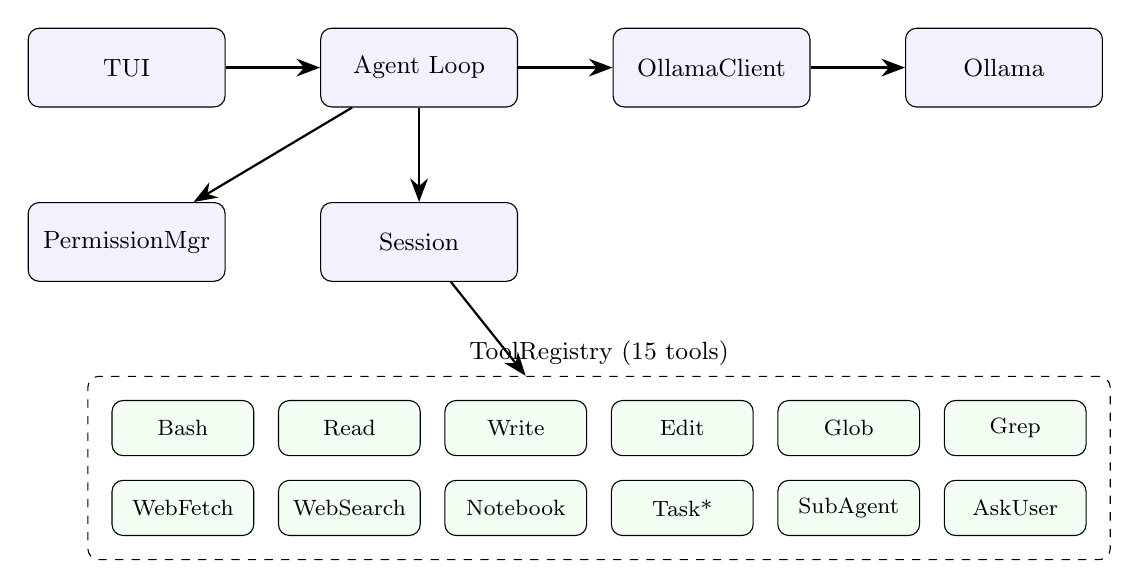
\begin{tikzpicture}[
  box/.style={draw, rounded corners, minimum height=1cm, minimum width=2.5cm, fill=blue!5, font=\small},
  tool/.style={draw, rounded corners, minimum height=0.7cm, minimum width=1.8cm, fill=green!5, font=\footnotesize},
  arr/.style={-{Stealth[length=3mm]}, thick},
  node distance=1.2cm
]
  % Main components
  \node[box] (tui) {TUI};
  \node[box, right=of tui] (agent) {Agent Loop};
  \node[box, right=of agent] (client) {OllamaClient};
  \node[box, right=of client] (ollama) {Ollama};

  % Session and Permissions
  \node[box, below=of agent] (session) {Session};
  \node[box, left=of session] (perm) {PermissionMgr};

  % Tools
  \node[tool, below=1.5cm of session, xshift=-3cm] (bash) {Bash};
  \node[tool, right=0.3cm of bash] (read) {Read};
  \node[tool, right=0.3cm of read] (write) {Write};
  \node[tool, right=0.3cm of write] (edit) {Edit};
  \node[tool, right=0.3cm of edit] (glob) {Glob};
  \node[tool, right=0.3cm of glob] (grep) {Grep};

  \node[tool, below=0.3cm of bash] (web) {WebFetch};
  \node[tool, right=0.3cm of web] (search) {WebSearch};
  \node[tool, right=0.3cm of search] (nb) {Notebook};
  \node[tool, right=0.3cm of nb] (task) {Task*};
  \node[tool, right=0.3cm of task] (sub) {SubAgent};
  \node[tool, right=0.3cm of sub] (ask) {AskUser};

  % Tool registry box
  \node[draw, dashed, rounded corners, fit=(bash)(read)(write)(edit)(glob)(grep)(web)(search)(nb)(task)(sub)(ask), inner sep=0.3cm, label={[font=\small]above:ToolRegistry (15 tools)}] (registry) {};

  % Arrows
  \draw[arr] (tui) -- (agent);
  \draw[arr] (agent) -- (client);
  \draw[arr] (client) -- (ollama);
  \draw[arr] (agent) -- (session);
  \draw[arr] (agent) -- (perm);
  \draw[arr] (session) -- (registry);

\end{tikzpicture}
\caption{vibe-coder architecture: 9 core classes with 15 integrated tools.}
\end{figure}

\subsection{Core Classes}

Table~\ref{tab:classes} summarizes the 9 core classes.

\begin{table}[h]
\centering
\caption{Core classes in vibe-coder.py}
\label{tab:classes}
\begin{tabular}{@{}llr@{}}
\toprule
\textbf{Class} & \textbf{Responsibility} & \textbf{$\sim$Lines} \\
\midrule
\texttt{Config} & CLI args, config file, env vars, model routing & 150 \\
\texttt{OllamaClient} & Ollama API (SSE streaming, function calling, retries) & 250 \\
\texttt{Tool} (base) & Abstract interface for all 15 tools & 30 \\
\texttt{ToolRegistry} & Tool dispatch, OpenAI schema generation & 100 \\
\texttt{PermissionMgr} & Permission rules (safe/ask/deny), pattern matching & 200 \\
\texttt{Session} & Message history, token estimation, compaction & 400 \\
\texttt{Agent} & Agentic loop: LLM $\to$ tool $\to$ result $\to$ loop & 350 \\
\texttt{TUI} & Terminal UI, readline, ANSI, streaming, CJK & 500 \\
\texttt{main()} & Entrypoint, Ollama connectivity, model selection & 200 \\
\bottomrule
\end{tabular}
\end{table}

\subsection{Tool Inventory}

\begin{table}[h]
\centering
\caption{15 integrated tools with permission classification}
\label{tab:tools}
\begin{tabular}{@{}llll@{}}
\toprule
\textbf{Tool} & \textbf{Category} & \textbf{Permission} & \textbf{Description} \\
\midrule
BashTool & Execution & ask & Shell commands, timeout, background \\
ReadTool & File I/O & safe & Text, images (base64), PDF, notebook \\
WriteTool & File I/O & ask & Atomic write via \texttt{mkstemp}+\texttt{os.replace} \\
EditTool & File I/O & ask & Search-replace with uniqueness check \\
GlobTool & Search & safe & \texttt{os.walk} + \texttt{fnmatch}, mtime-sorted \\
GrepTool & Search & safe & Regex search, context lines, output modes \\
WebFetchTool & Network & ask & URL fetch, HTML$\to$text, charset detect \\
WebSearchTool & Network & ask & DuckDuckGo HTML scraping, CJK locale \\
NotebookEditTool & File I/O & ask & Jupyter \texttt{.ipynb} cell editing \\
TaskCreateTool & Task mgmt & safe & Create tracked tasks \\
TaskListTool & Task mgmt & safe & List all tasks \\
TaskGetTool & Task mgmt & safe & Get task details \\
TaskUpdateTool & Task mgmt & safe & Update task status \\
SubAgentTool & Agent & ask & Spawn sub-agent (read-only, max 20 turns) \\
AskUserQuestionTool & UX & safe & Prompt user for clarification \\
\bottomrule
\end{tabular}
\end{table}

\subsection{Agentic Loop}

The core agent loop follows a standard ReAct~\cite{yao2023react} pattern:

\begin{lstlisting}[language=Python, caption={Simplified agent loop}]
def run(self, user_input):
    self.session.add_user_message(user_input)
    while not self._interrupted:
        # 1. Stream LLM response
        response = self.client.chat(
            model=self.model,
            messages=self.session.get_messages(),
            tools=self.registry.get_schemas(),
            stream=True)
        text, tool_calls = self.tui.stream_response(response)

        # 2. XML fallback for models without function calling
        if not tool_calls and text:
            tool_calls = extract_tool_calls_from_text(text)

        self.session.add_assistant_message(text, tool_calls)
        if not tool_calls:
            break

        # 3. Execute tools (parallel for safe tools)
        results = self._execute_tools(tool_calls)
        self.session.add_tool_results(results)

        # 4. Context compaction if needed
        self.session.compact_if_needed()
\end{lstlisting}

\paragraph{XML Fallback.}
Many local LLMs (especially Qwen-family models) sometimes emit tool calls as XML rather than structured function calling.
We implement a robust XML extraction pipeline with:
entity decoding,
ReDoS bail-out for pathological patterns,
JSON auto-parsing of arguments,
known-tool filtering, and
deduplication with JSON-normalized comparison.

\paragraph{Parallel Tool Execution.}
Safe tools (Read, Glob, Grep) are executed in parallel using \texttt{ThreadPoolExecutor}, with results buffered and displayed in call order to maintain deterministic output.

\subsection{Context Management}

Local LLMs typically have smaller context windows (4K--128K tokens) compared to cloud models.
vibe-coder implements a multi-layered context management strategy:

\begin{enumerate}[nosep]
  \item \textbf{Token estimation}: CJK-aware character counting with expanded Unicode ranges (CJK Unified, Extension A, Hiragana, Katakana, fullwidth forms, Korean syllables).
  \item \textbf{Explicit \texttt{num\_ctx}}: The \texttt{options.num\_ctx} parameter is sent in every Ollama API call to ensure server-side context window matches client-side tracking.
  \item \textbf{Automatic compaction}: At 70\% context utilization, older messages are summarized using a sidecar model while preserving the most recent 30 message pairs.
  \item \textbf{Tool result truncation}: Large tool outputs are truncated at 50{,}000 characters with a notice.
  \item \textbf{Max messages}: Hard cap at 500 messages with FIFO eviction preserving tool-call/result pairing.
\end{enumerate}

\subsection{Security Model}

Security is designed in depth with multiple layers:

\begin{table}[h]
\centering
\caption{Security measures by category}
\label{tab:security}
\begin{tabular}{@{}lp{10cm}@{}}
\toprule
\textbf{Category} & \textbf{Measures} \\
\midrule
Path traversal & Symlink resolution (\texttt{os.path.realpath}), protected path blocking (\texttt{/etc/passwd}, \texttt{/etc/shadow}, \texttt{.ssh/}), 10MB/50MB file size limits \\
SSRF & IP validation (private ranges, link-local, IPv4-mapped IPv6), DNS fail-closed, redirect host checking, localhost-only Ollama host \\
Injection & Environment variable sanitization (allowlist core + denylist secrets), dangerous command blocking (\texttt{rm -rf /}, \texttt{eval}, \texttt{base64 -d | sh}), prompt injection resistance \\
Atomic writes & All file operations use \texttt{tempfile.mkstemp} + \texttt{os.replace} for crash safety \\
Subprocess & \texttt{stdin=DEVNULL}, \texttt{start\_new\_session=True}, process group kill on timeout, zombie prevention \\
\bottomrule
\end{tabular}
\end{table}

\section{Iterative Development Methodology}

\subsection{AI-Assisted Multi-Agent Audit}

A distinguishing feature of vibe-coder's development is the use of \textbf{parallel AI agent audits} for systematic code review.
In each round, 3--40 specialized agents were launched concurrently, each focused on a specific concern (security, reliability, UX, testing, performance, etc.).
Their findings were triaged, cross-referenced against the current codebase, and applied in batch.

\begin{table}[h]
\centering
\caption{Development rounds and cumulative metrics}
\label{tab:rounds}
\begin{tabular}{@{}clrrr@{}}
\toprule
\textbf{Round} & \textbf{Focus} & \textbf{Fixes} & \textbf{Tests} & \textbf{Lines} \\
\midrule
1 & Foundation (20 agents) & 29 & -- & $\sim$1500 \\
2 & Robustness (16 agents) & 15 & -- & $\sim$2000 \\
2.5 & Edge cases & 8 & -- & $\sim$2200 \\
3 & IME + LLM + UX & 16 & -- & $\sim$2500 \\
4 & Deep audit (40 agents) & 23 & -- & $\sim$2800 \\
5 & Comprehensive (20 agents) & 21 & -- & $\sim$3200 \\
6 & Feature parity & 21 & 119 & $\sim$3500 \\
7 & Security + reliability (4 agents) & 29 & 160 & $\sim$3800 \\
8 & Features + critical fixes (5 agents) & 22 & 384 & $\sim$4600 \\
9 & Robustness + UX & 20+ & 432 & $\sim$4770 \\
10 & File/TUI/Ollama audit & 20+ & 459 & $\sim$4916 \\
11 & Security deep audit & 12 & 477 & $\sim$5000 \\
12 & Agent loop + install hardening & 15+ & 542 & 5399 \\
\bottomrule
\end{tabular}
\end{table}

\subsection{Methodology Details}

Each audit round follows a consistent process:

\begin{enumerate}[nosep]
  \item \textbf{Agent deployment}: Launch $N$ parallel agents with specific audit charters (e.g., ``find all SSRF vectors'', ``audit symlink handling'', ``test CJK display width'').
  \item \textbf{Report collection}: Each agent produces a structured report with severity classifications (Critical, High, Medium, Low).
  \item \textbf{Triage}: Cross-reference findings against current codebase; eliminate false positives and already-fixed issues.
  \item \textbf{Implementation}: Apply fixes in dependency order (critical first, then high, medium, low).
  \item \textbf{Validation}: Run full test suite after each batch; add regression tests for each fix.
  \item \textbf{Documentation}: Update review-plan.md with applied fixes and updated metrics.
\end{enumerate}

The multi-agent approach provides several advantages over sequential review:
\begin{itemize}[nosep]
  \item \textbf{Coverage}: Each agent explores a different concern axis, reducing blind spots.
  \item \textbf{Speed}: Parallel execution completes in the time of the slowest agent rather than the sum.
  \item \textbf{Diversity}: Different agent prompts surface different classes of issues.
  \item \textbf{Regression}: Accumulated tests prevent fix regressions across rounds.
\end{itemize}

\section{CJK and Internationalization}

\subsection{Terminal Display Width}

CJK characters occupy two terminal columns, while Latin characters occupy one.
Standard \texttt{len()} is insufficient for terminal layout.
We implement \texttt{\_display\_width()} using Unicode East Asian Width properties:

\begin{lstlisting}[language=Python, caption={CJK-aware display width calculation}]
def _display_width(text):
    w = 0
    for ch in text:
        eaw = unicodedata.east_asian_width(ch)
        w += 2 if eaw in ('W', 'F') else 1
    return w
\end{lstlisting}

\subsection{Japanese IME Support}

Japanese input via IME (Input Method Editor) requires double-Enter confirmation.
The first Enter confirms the IME composition; the second submits the input.
We detect CJK locales and adjust readline behavior accordingly.

\subsection{Search Localization}

DuckDuckGo searches are localized with the \texttt{kl} parameter (e.g., \texttt{kl=jp-ja} for Japanese) and \texttt{Accept-Language} headers, detected automatically from the system locale.

\subsection{Permission Dialog Localization}

Permission prompts accept Japanese responses: \begin{CJK}{UTF8}{min}常に\end{CJK} (always), \begin{CJK}{UTF8}{min}いいえ\end{CJK} (no), \begin{CJK}{UTF8}{min}拒否\end{CJK} (deny), alongside English equivalents.

\section{User Testing and Bug Reports}

\subsection{Case Study: Windows PowerShell (Issue \#4)}

A user (\texttt{rara2022}) reported two issues on Windows:

\paragraph{Bug 1: \texttt{\$Debug} Parameter Collision.}
PowerShell reserves \texttt{\$Debug} as a common parameter.
Our launcher script (\texttt{vibe-local.ps1}) used \texttt{[switch]\$Debug}, causing a conflict:
\begin{verbatim}
A parameter with the name 'Debug' was defined multiple times
\end{verbatim}
\textbf{Fix}: Renamed to \texttt{\$DebugMode} with corresponding internal variable updates.

\paragraph{Bug 2: \texttt{Invoke-RestMethod} Failure.}
The Ollama connectivity check used \texttt{Invoke-RestMethod}, which fails when the response is not valid JSON (Ollama's \texttt{/api/tags} can return unexpected formats).
\textbf{Fix}: Replaced with \texttt{Invoke-WebRequest -UseBasicParsing} (checks HTTP status only) with a TCP socket fallback:

\begin{lstlisting}[language=bash, caption={Robust Ollama detection on Windows}]
try {
    $resp = Invoke-WebRequest -Uri "$OllamaHost/api/tags" `
        -TimeoutSec 3 -UseBasicParsing -ErrorAction Stop
    return ($resp.StatusCode -eq 200)
} catch {
    # Fallback: TCP connection test
    $tcp = New-Object System.Net.Sockets.TcpClient
    $tcp.Connect($uri.Host, $uri.Port)
    $tcp.Close()
    return $true
}
\end{lstlisting}

\subsection{Findings from User Testing}

Key insights from user interaction and bug reports:
\begin{enumerate}[nosep]
  \item \textbf{Platform-specific pitfalls}: PowerShell reserved parameters and API behavior differences are not caught by Unix-only testing.
  \item \textbf{Error message clarity}: Beginner users need actionable error messages with copy-pasteable commands (e.g., ``\texttt{ollama pull qwen3:8b}'').
  \item \textbf{Installer robustness}: Package manager differences (Homebrew, apt, pacman, winget) require extensive platform detection.
  \item \textbf{CJK display}: Banner art and separators must use Na-width characters to avoid misalignment on CJK terminals.
  \item \textbf{Permission UX}: Users in non-English locales expect localized permission responses.
\end{enumerate}

\section{Performance Considerations}

\subsection{Startup Optimization}

We applied 10 performance fixes to minimize startup latency:
\begin{itemize}[nosep]
  \item \texttt{GlobTool}: Primary \texttt{os.walk} instead of \texttt{Path.rglob} (avoids stat overhead).
  \item Schema caching: Tool schemas generated once at registry initialization.
  \item Deduplicated startup checks (single Ollama connectivity probe).
  \item Banner-first display (user sees output before model validation).
  \item \texttt{GrepTool}: Binary file probe (skip files $>$50MB or with null bytes).
\end{itemize}

\subsection{Context Compaction Accuracy}

Compaction preserves tool-call/result pairing integrity.
Orphaned tool results (tool results without matching tool calls) are detected and removed during compaction to prevent LLM confusion.

\section{Comparison with Existing Tools}

\begin{table}[h]
\centering
\caption{Feature comparison with commercial coding assistants}
\label{tab:comparison}
\begin{tabular}{@{}lcccc@{}}
\toprule
\textbf{Feature} & \textbf{vibe-coder} & \textbf{Claude Code} & \textbf{aider} & \textbf{Continue} \\
\midrule
Offline operation & \checkmark & -- & -- & -- \\
No cloud account & \checkmark & -- & -- & -- \\
Single file & \checkmark & -- & -- & -- \\
Stdlib only & \checkmark & -- & -- & -- \\
Agentic loop & \checkmark & \checkmark & Partial & Partial \\
Tool use (15+) & \checkmark & \checkmark & Partial & Partial \\
CJK support & \checkmark & Partial & -- & -- \\
Context compaction & \checkmark & \checkmark & \checkmark & -- \\
Session persistence & \checkmark & \checkmark & \checkmark & -- \\
SubAgent & \checkmark & \checkmark & -- & -- \\
Image support & \checkmark & \checkmark & -- & Partial \\
PDF reading & \checkmark & \checkmark & -- & -- \\
Task management & \checkmark & \checkmark & -- & -- \\
Plan mode & \checkmark & \checkmark & -- & -- \\
Auto model pull & \checkmark & N/A & -- & -- \\
\bottomrule
\end{tabular}
\end{table}

\section{Future Directions}

\subsection{Short-term (v1.0)}

\begin{itemize}[nosep]
  \item \textbf{MCP Client}: Model Context Protocol support for external tool servers.
  \item \textbf{Persistent permissions}: Save per-project permission rules across sessions.
  \item \textbf{Rich diff preview}: Side-by-side colored diff display for Edit operations.
  \item \textbf{Type annotations}: Full type hints for IDE support and static analysis.
  \item \textbf{/doctor command}: Self-diagnostic tool checking Ollama, model availability, and system configuration.
\end{itemize}

\subsection{Medium-term}

\begin{itemize}[nosep]
  \item \textbf{Multi-model orchestration}: Route different tasks to different models (e.g., small model for Glob, large for code generation).
  \item \textbf{Hooks system}: User-defined pre/post hooks for tool execution.
  \item \textbf{Plugin architecture}: Loadable tool plugins without modifying the main file.
  \item \textbf{VS Code extension}: Integration as an IDE extension (language server protocol).
  \item \textbf{Benchmark suite}: Standardized coding task benchmarks for model comparison.
\end{itemize}

\subsection{Research Directions}

\begin{itemize}[nosep]
  \item \textbf{Compaction quality}: How does summarization quality affect long-session accuracy? Can smaller models produce adequate summaries?
  \item \textbf{Tool selection accuracy}: How do different local models compare in tool-use accuracy? What prompt engineering techniques improve reliability?
  \item \textbf{CJK token efficiency}: Local models have varying CJK tokenization; how does this affect context utilization?
  \item \textbf{Offline knowledge}: Without web search, how can local RAG (retrieval-augmented generation) supplement model knowledge?
\end{itemize}

\section{Conclusion}

vibe-coder demonstrates that a production-quality coding agent can be built as a single Python file with zero external dependencies.
Through 12 rounds of iterative AI-assisted auditing, we achieved 155+ fixes and 542 tests while maintaining the single-file, stdlib-only constraint.
The project validates a development methodology where parallel AI agents systematically audit different concern axes, with human oversight for triage and integration.

The system is freely available, fully offline-capable, and designed for global accessibility---including first-class support for CJK languages that are underserved by existing tools.
We believe this approach---radical simplicity combined with rigorous iterative refinement---offers a viable path toward democratizing AI-powered development tools.

\begin{thebibliography}{9}

\bibitem{anthropic2024}
Anthropic. \textit{Claude Code CLI}. \url{https://docs.anthropic.com/}, 2024--2025.

\bibitem{yao2023react}
S. Yao, J. Zhao, D. Yu, et al.
``ReAct: Synergizing Reasoning and Acting in Language Models.''
\textit{ICLR}, 2023.

\bibitem{ollama2024}
Ollama. \textit{Ollama: Run large language models locally}. \url{https://ollama.com/}, 2024.

\bibitem{duckduckgo}
DuckDuckGo. \textit{DuckDuckGo HTML Search}. \url{https://duckduckgo.com/}, 2024.

\end{thebibliography}

\end{document}
